\chapter{The classical methods: Wiener, ISTA, FISTA}\label{ch:classics}

Every network here is built from these three ideas, so they come first.

\section{What is Wiener?}

You asked about this directly. The Wiener filter in our tables is the simplest sensible way to undo
the blur. It involves no learning at all.

We want an image $x$ whose blurred version matches $b$, but we refuse to let $x$ get too large:
\begin{equation}
\min_x\; \lVert h * x - b \rVert_2^2 + \mu \lVert x \rVert_2^2 .
\end{equation}
The first term says ``match the measurement''. The second says ``keep it small''. In Fourier space
each frequency is a separate small problem, and setting the derivative to zero gives the answer directly:
\begin{equation}
\widehat{x}(f) = \frac{h(f)}{h(f)^2 + \mu}\; \widehat{b}(f).
\end{equation}

Look at what this does. Where $h$ is large (slow patterns), $\mu$ is negligible, so the fraction is
about $1/h$: a true inverse. Where $h$ is tiny, the fraction is about $h/\mu$, which goes to zero.
So it inverts what it can trust and gives up on the rest. The blue line in
Figure~\ref{fig:filters} shows this.

\begin{code*}{csc_lista.py}
class Dataless(nn.Module):
    """Tikhonov/Wiener baseline with the same exp(-kz) operator."""

    def __init__(self, dx, dz, mu):
        super().__init__()
        self.dx, self.dz, self.mu = dx, dz, mu

    def forward(self, b):
        n = b.shape[-1]
        h = transfer(n, self.dx, self.dz, b.dtype, b.device)
        return torch.fft.irfft2(torch.fft.rfft2(b) * h / (h * h + self.mu), s=(n, n))
\end{code*}

The only setting is $\mu$. We tried values from $10^{-6}$ to $10^{-0.5}$ in half-decade steps on
simulated validation crops, and $\mu=0.0316$ won. With this $\mu$ the largest gain is 2.8, at a
period of about 9\um. Beyond about 0.4 cycles per \textmu m its gain is below 0.1, so it has effectively given up.

Strictly, a true Wiener filter uses the signal and noise spectra. With a single constant $\mu$
this is also called \textbf{Tikhonov} regularisation. The code's docstring says both, and the
tables use the short name Wiener.

\begin{keyidea}[Why Wiener matters here]
It is the honest baseline. It knows the physics, uses no training data, and takes one line. Any network
must beat it. It scores 49.3\% on COMSOL.
\end{keyidea}

\section{Sparse coding: a better belief}

Wiener treats every frequency separately, so it cannot know that fields come from wires. Sparse
coding says something stronger: \emph{a sharp field is made of a few repeated pieces}.

Take a set of small images $g_1,\dots,g_M$, called \textbf{atoms}, or together a
\textbf{dictionary}. Stamp them at chosen positions and add them up:
\begin{equation}
t \approx \sum_{m=1}^{M} g_m * x_m .
\end{equation}
Each $x_m$ is a map the size of the image, called a \textbf{code}. Most of its values are zero, and a
nonzero value means ``stamp atom $m$ here, this strongly''.

\begin{keyidea}[The trick that puts the blur in]
We measure $b = h*t$. Substitute the sparse model for $t$:
\begin{equation}
b \approx h * \sum_m g_m * x_m = \sum_m (h * g_m) * x_m = \sum_m d_m * x_m,
\qquad d_m = h*g_m .
\end{equation}
So the \textbf{blurred} field is built from \textbf{blurred} atoms $d_m$, using the \emph{same} codes. Find
the codes from $b$ using $d$, then rebuild the sharp field using $g$. That is the whole method.
\end{keyidea}

\begin{center}
\begin{tikzpicture}[node distance=6mm and 11mm]
\node[fixed] (b) {Blurry $b$};
\node[block,right=of b] (solve) {Find sparse codes $x$\\ so that $\sum d_m*x_m\approx b$};
\node[block,right=of solve] (rebuild) {Rebuild\\ $y=\sum g_m*x_m$};
\node[fixed,right=of rebuild] (y) {Sharp $y$};
\draw[flow] (b) -- (solve);
\draw[flow] (solve) -- (rebuild);
\draw[flow] (rebuild) -- (y);
\end{tikzpicture}
\end{center}

To find the codes, we solve the \textbf{Lasso}:
\begin{equation}
\min_x\; \tfrac12 \Big\lVert \sum_m d_m*x_m - b \Big\rVert_2^2 + \lambda \lVert x \rVert_1 .
\end{equation}
The first term matches the measurement. The second, the $\ell_1$ penalty, pushes values to exactly
zero. A larger $\lambda$ gives sparser codes and a worse fit.

\section{ISTA}

ISTA solves the Lasso by repeating two simple moves. Write $D$ for the operator
$x\mapsto\sum_m d_m*x_m$ and $D^T$ for its transpose.

\begin{equation}
x^{(k+1)} = \soft_{\lambda/L}\!\left( x^{(k)} - \frac1L D^T\big(Dx^{(k)} - b\big) \right).
\end{equation}

\begin{enumerate}
\item \textbf{Gradient step.} $Dx-b$ is the current mismatch. $D^T$ carries it back to code space. We
step downhill by $1/L$. $L$ must be at least the largest eigenvalue of $D^TD$, or the iteration can
blow up.
\item \textbf{Shrink.} The function $\soft_\theta$ moves every value toward zero by $\theta$, and small values
land exactly on zero. This is where sparsity comes from.
\end{enumerate}

\begin{minipage}{.5\textwidth}
\begin{code*}{csc_lista.py}
def shrink(x, theta):
    return torch.sign(x) * torch.relu(torch.abs(x) - theta)
\end{code*}
\end{minipage}\hfill
\begin{minipage}{.44\textwidth}
\centering
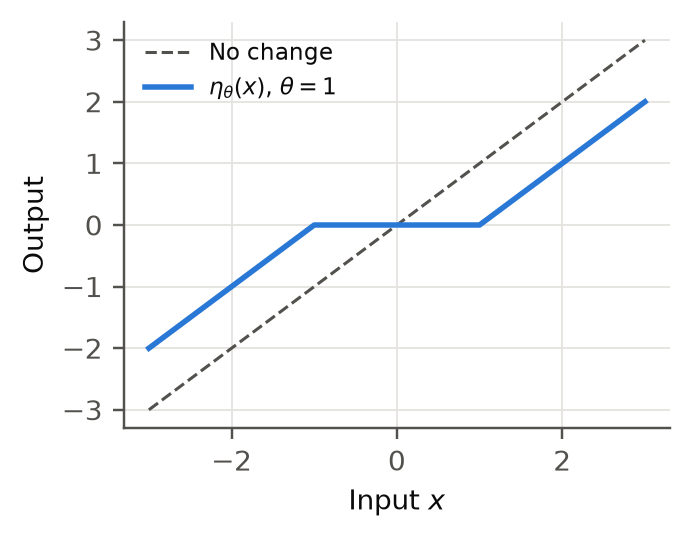
\includegraphics[width=\linewidth]{shrink}
\captionof{figure}{Soft thresholding. Anything within $\pm\theta$ becomes zero.}
\end{minipage}

\medskip
In formula form, $\soft_\theta(x)=\sign(x)\max(|x|-\theta,0)$. The code is that formula.

\section{FISTA}

ISTA is slow. FISTA adds one small idea, momentum. It takes the gradient step not from the
current point, but from a point pushed further along the direction it was already moving:
\begin{align}
x^{(k)} &= \soft_{\lambda/L}\!\left( y^{(k)} - \tfrac1L D^T(Dy^{(k)} - b) \right),\\
t_{k+1} &= \tfrac12\big(1+\sqrt{1+4t_k^2}\big),\\
y^{(k+1)} &= x^{(k)} + \frac{t_k-1}{t_{k+1}}\big(x^{(k)}-x^{(k-1)}\big).
\end{align}
The cost per step is the same, but the convergence rate improves from $O(1/k)$ to $O(1/k^2)$. Our code holds
both algorithms in one function, with \code{fast} choosing between them:

\begin{code*}{csc_lista.py}
def code_ista(b, operator, lam, steps, pad=0, fast=True, bound=None):
    """FISTA or ISTA for 0.5 ||mask(Dx - b)||^2 + lam ||x||_1."""
    n = b.shape[-1]
    mask = window_mask(n, pad, b.device) if pad else 1.0
    step = 1 / (bound or operator.bound(n))
    x = torch.zeros(b.shape[0], operator.filters.shape[0], n, n, dtype=b.dtype,
                    device=b.device)
    y, t = x, 1.0
    for _ in range(steps):
        residual = mask * (operator.forward(y) - b)
        update = shrink(y - step * operator.adjoint(residual), lam * step)
        if fast:
            t_next = (1 + (1 + 4 * t * t) ** .5) / 2
            y = update + (t - 1) / t_next * (update - x)
            t = t_next
        else:
            y = update
        x = update
    return x
\end{code*}

\section{How well do they do?}

Both use the same dictionary as the networks. FISTA's $\lambda$ was picked on 16 simulated validation crops. The first
search tried 0.03, 0.09, 0.3 and 0.9, and the smallest won. That is the edge of the grid, so the search was widened, and
$\lambda=0.009$ won with worse values on both sides. Chapter~\ref{ch:results} shows the full search.

\begin{center}
\begin{tabular}{lcc}
\toprule
Method & Simulated validation & COMSOL \\
\midrule
ISTA, 16 iterations & 64.3\% & 64.4\% \\
FISTA, 32 iterations & 50.9\% & 41.8\% \\
FISTA, 64 iterations & 45.3\% & 37.9\% \\
FISTA, 300 iterations, $\lambda=0.03$ & 36.6\% & 32.1\% \\
FISTA, 300 iterations, $\lambda=0.009$ & 35.5\% & 30.5\% \\
\bottomrule
\end{tabular}
\end{center}

\begin{keyidea}[Read this table carefully]
ISTA with 16 steps is awful because it has barely started. FISTA with 300 steps is the best thing in
the whole project so far. So the sparse model itself is good, and the problem is speed. This is exactly
what learned networks were invented to fix: reach a similar answer in far fewer steps.
\end{keyidea}
